\documentclass{article}

\usepackage{pgfplots}
\usepackage{tikz}

\begin{document}

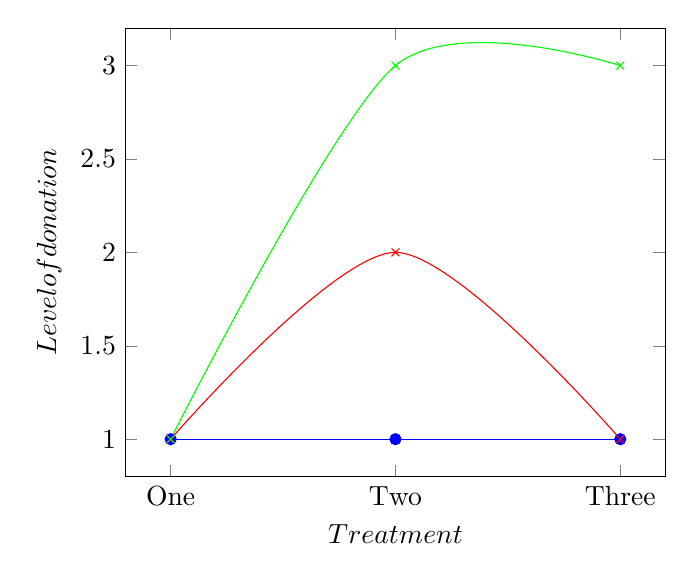
\begin{tikzpicture}
% \pgfplotsset{ticks=none}
\begin{axis}[
legend style={at={(1,1)},anchor=north west},
xtick={1,2,3},
xticklabels={One,Two,Three},
xlabel=$Treatment$,
ylabel=$Level of donation$]
\addplot[smooth,mark=*,blue] plot coordinates {
    (1,1)
    (2,1)
    (3,1)
};
%\addlegendentry{Pure Altruism}

\addplot[smooth,color=red,mark=x]
plot coordinates {
    (1,1)
    (2,2)
    (3,1)
};
%\addlegendentry{Warm Glow}

\addplot[smooth,color=green,mark=x]
plot coordinates {
    (1,1)
    (2,3)
    (3,3)
};
%\addlegendentry{Mental Accounting}
\end{axis}
\end{tikzpicture}

\end{document}